\section{Introduction}
\label{introduction}

The physics program for CLAS12 in Jefferson Lab's Hall B requires the use of electron beams of various energies and currents that impinge
upon on targets ranging from liquid hydrogen to lead. A significant part of the physics program includes running with polarized targets that 
require a rastered beam on the target. In order to extract experimental observables, accurate measurements of the beam charge and 
polarization are required. Also, for safe and efficient operation of a large, open acceptance spectrometer, proper shielding and a stable beam 
with a small lateral size and minimal beam halo are needed. 

The Hall-B beamline is designed to satisfy experimental requirements and provide necessary controls and monitoring 
of the electron beam properties for safe and efficient operation of CLAS12. The key set of parameters required by experiments with CLAS12 
is listed in Table \ref{tab:beam_par}. The main challenges for the beamline setup are the open acceptance of CLAS12 and the close proximity 
of various sensitive detectors to the target and beam. Such challenges were successfully overcome in Hall B in the past for CLAS \cite{CLAS} 
experiments and the Heavy Photon Search (HPS) experiment \cite{HPS}.

 \begin{table}[htb]
 \centering
 \begin{tabular}{|c|c|c|}
\hline
Parameter & Requirement &Unit \\ \hline 
$E$ &  $\le 11$& GeV \\ \hline
$\delta p/p$ & $< 10^{-4}$ & \\ \hline 
Current & $50$ to $500$ & nA \\ \hline
Current instability & $\sim 10$ &\% \\ \hline 
$\sigma_x $, $\sigma_y$&$< 300$& $\mu$m \\ \hline 
Position stability &$< 200$ &$\mu$m \\ \hline
Divergence& $< 100$& $\mu$rad \\ \hline 
Beam halo ($> 5\sigma$) &$< 10^{-4}$& \\ \hline
Beam polarization &$> 0.85$& \\ \hline
\end{tabular}
\caption{Nominal required Hall B beam parameters.} 
\label{tab:beam_par}
\end{table}

A few key modifications to the beamline \cite{HPSBeamline} used during the lower-energy run of the HPS experiment have been introduced 
in order to establish high-quality physics beams in Hall B and run CLAS12 at the design luminosity of $10^{35}$ cm$^{-2}$s$^{-1}$.  
Additions to the beamline for high-energy running of CLAS12 include a new intermediate beam dump upstream of the hall, a cryogenic 
target system, shielding downstream of the target to protect CLAS12 detectors from electromagnetic backgrounds, and the M{\o}ller 
polarimeter for beam polarization measurements.   

%\begin{figure*}[t]
%\begin{center}
%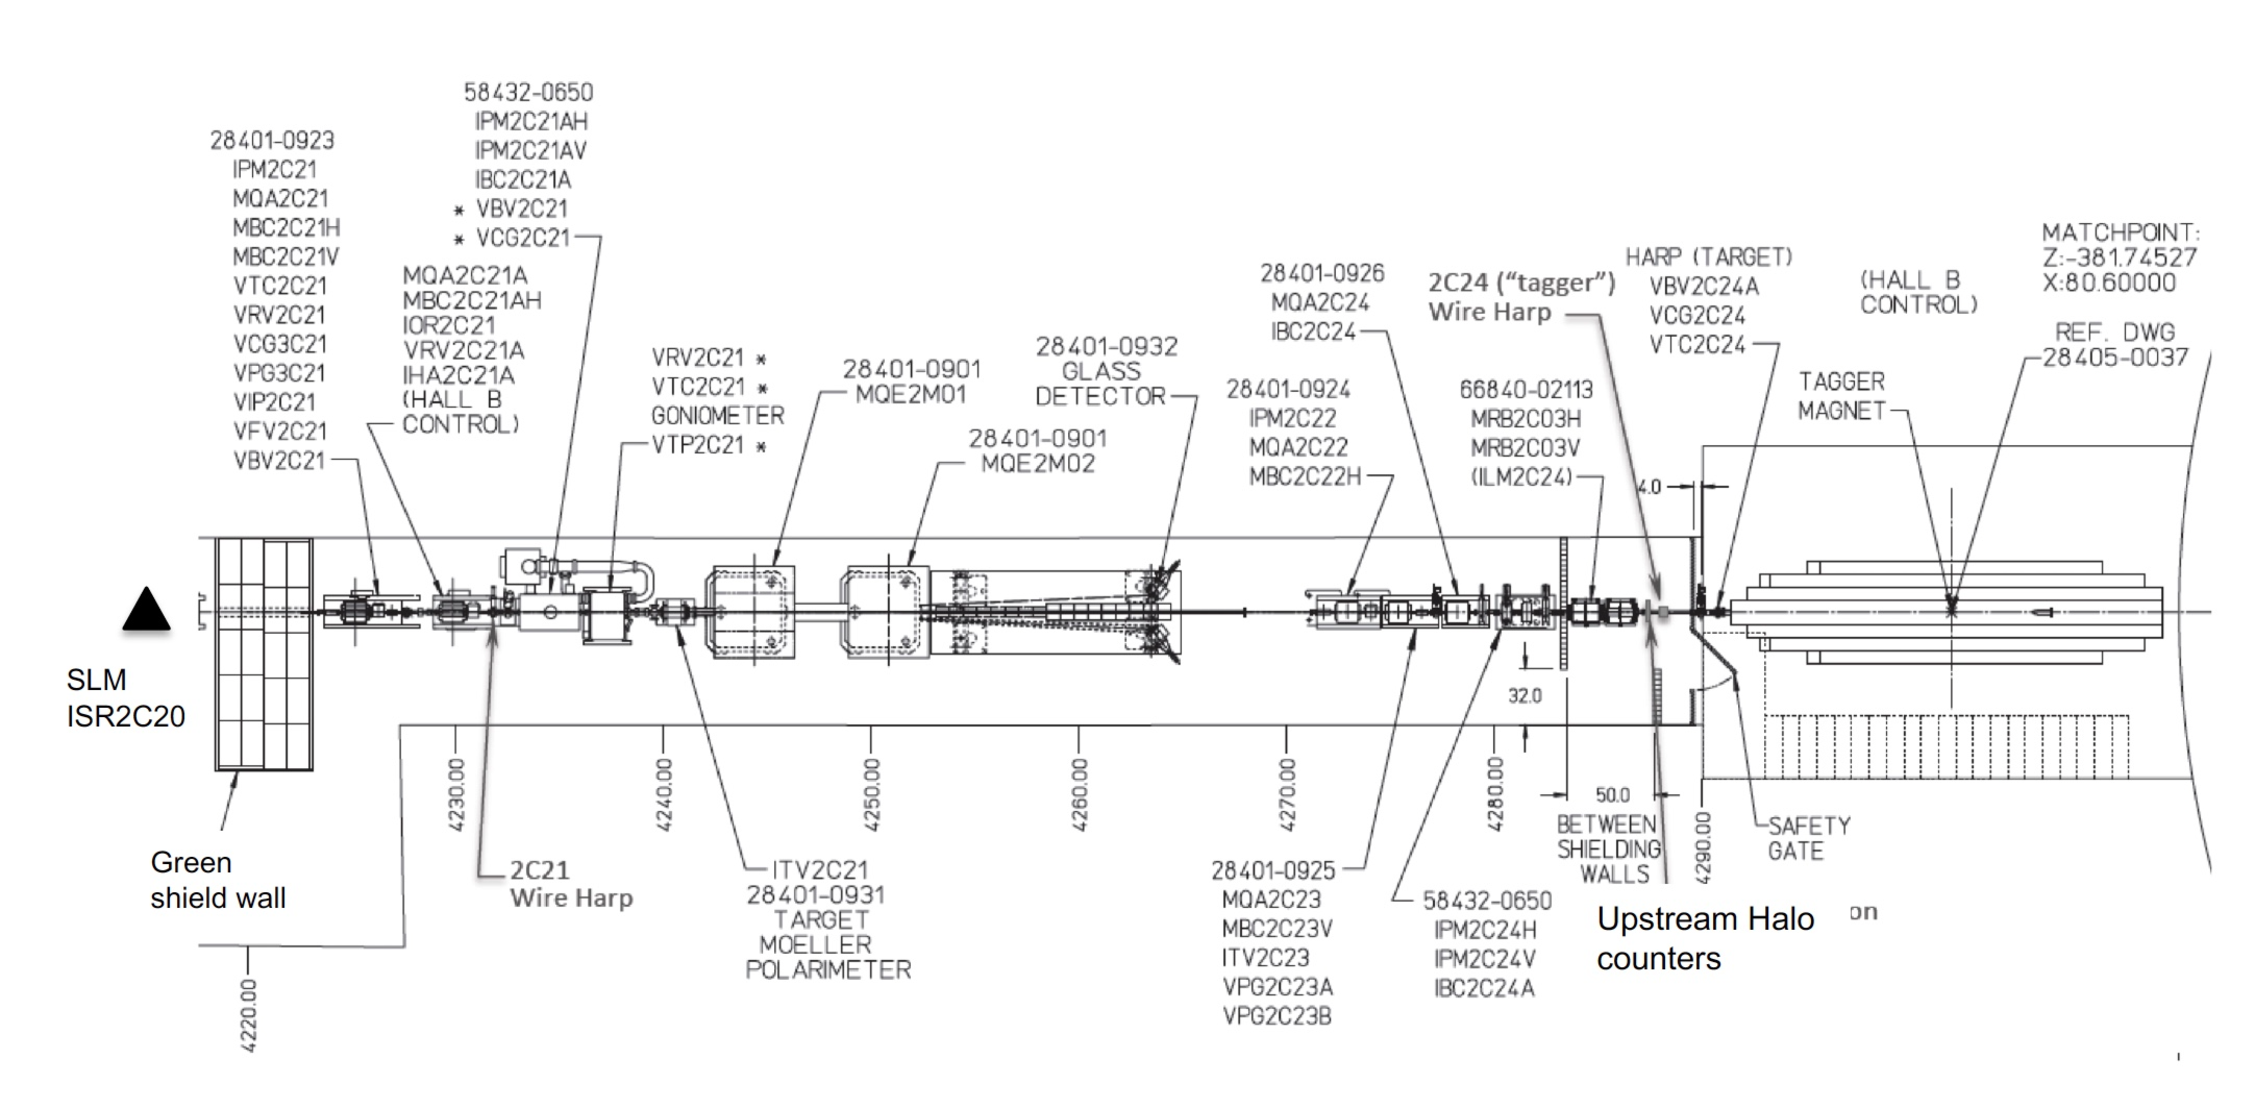
\includegraphics[width=1.\textwidth]{upstream_tunnel.pdf}
%\caption{Overhead view of the 2C beamline in the tunnel upstream of Hall B. {\color{red} Not the final figure.}}
%\label{fig:upstream}
%\end{center}
%\end{figure*}

 
This paper will discuss the design of the Hall-B beamline for CLAS12, and its performance during the 2018 experimental run. It will review the 
beamline instrumentation used to measure and monitor beam parameters and to protect CLAS12 detectors against errant beam motion. As will 
be demonstrated, excellent quality and stability of the CEBAF beams, coupled with the Hall-B beamline protection systems, allowed running the 
CLAS12 detector at the design luminosity.


